% this file is called up by thesis.tex
% content in this file will be fed into the main document

%: ----------------------- name of chapter  -------------------------
\chapter{Problem Statement} % top level followed by section, subsection

%transition between chapters, usually no more than two parragraphs

Conventional methods of displaying advertisements inside mobile applications usually feature a banner or full-screen interstitial, as seen on Figure \ref{fig:ads} \footnote[36]{http://googleadsdeveloper.blogspot.com/2011\_12\_01\_archive.html, 14.05.15} \footnote[37]{http://galleryhip.com/admob-ad.html, 14.05.15}.

\begin{figure}
\begin{center}
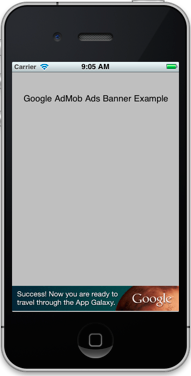
\includegraphics{Images/banner.png}
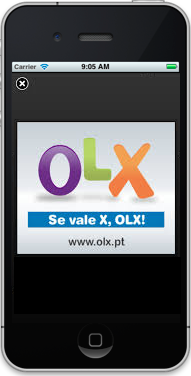
\includegraphics{Images/fullscreen.png}
\caption{Examples of advertisements}
\label{fig:ads}
\end{center}
\end{figure}

A banner advertisement is static and throughout the usage of an application takes up screen space that could otherwise host content of the application itself. In addition, banner advertisements are often flashing or making sound, further distracting the user from using the application.

Interstitial advertisements pop up from time to time throughout the usage of an application and temporarily stop the user from using the application altogether. Full-screen advertisements can be closed but it is often not intuitive how to do so without tapping on the advertisement itself and being redirected to the advertiser's website. In addition, opening and closing an interstitial advertisement often takes too long. it distracts the user and might get them out of the mood of using the application.

%: ----------------------- Mobile Cloud Middleware ------------------------

\section{Research Question}
%This section has three main parts: 
%1. a concise statement of the question that your thesis tackles 
%2. justification, by direct reference to section 3, that your question is previously unanswered
%3. discussion of why it is worthwhile to answer this question. 

The proposed solution for the problems that conventional advertising methods have, is to display advertisements to the user in a way that the user could choose the location and size of the advertisement on the screen. This thesis aims to evaluate whether this sort of mechanism is more user-friendly than mechanisms currently in use.

To do so, such a mechanism is developed and implemented for a mobile application as a proof of concept. People are then asked to compare it to conventional mobile advertising in terms of intrusiveness and their interest in the advertised product.

Advertisements are an inseparable part of mobile applications, but, as it stands, they are doing more harm than good. Users should feel that advertisements are a part of an application rather than an unwelcome addition. Research suggests that a high rate of exposure to advertisements has a negative impact on perceived advertising value\cite{parissa2005increasingadvalue}\cite{consumer2004melody}. If an application is usable without noticeable interruptions then the user can choose the pace at which they use the application and might pay more attention to the advertisements, since they can choose the time to do so.

%Summary of each chapter is MANDATORY
\section{Summary}
This thesis attempts to find a solution to many problems that conventional advertising mechanisms have. To counter the problems, a mechanism is developed that would allow displaying advertisements to the user in way that allows the user to choose the location and size of the advertisement on-screen. It is then implemented into a mobile application and users are asked to compare it to conventional advertising methods, to determine whether the proposed method makes the application better to use. The next describes the architecture of the created solution.